\documentclass[a4paper,12pt]{article}
\usepackage[margin=0.7in]{geometry}
\usepackage[latin1]{inputenc}
\usepackage[english]{babel}
\usepackage{amsmath}
\usepackage{cases}
\usepackage[makeroom]{cancel}
\usepackage{amsmath,tabu}
\usepackage[fleqn]{mathtools}
\usepackage[fleqn]{amsmath}
\usepackage{bm}
\usepackage{tikz}
\usepackage{enumitem}
\usepackage{wrapfig}
\usepackage{graphicx}
\usepackage{siunitx}
\usepackage{microtype}
\usepackage{array,tabularx}
\usepackage{float}
\usepackage{booktabs}
\usepackage{import}
\usepackage{cases}
\usepackage{graphicx,subfigure}
\usepackage{myUnitOfMeasure}
%\usepackage{myThermodynamics}
\usepackage{myMath}
\usepackage{mathtools}
\usepackage{gensymb}
\usepackage{xcolor}
\usepackage{url}
\usepackage{tabularx}
\usepackage{ltablex}
\usepackage{booktabs}
\usepackage{float}
\usepackage{listings}
\restylefloat{table} % with H force table position

\title{

\includegraphics[scale=0.4]{images/logo.png}
\\[1cm]
FINAL REPORT ON THE  MRL TURBINE SIMULATION
COURSE OF MODELING TECHNIQUES FOR FLUID MACHINES 
A.Y. 2017/2018}
\author{
Andrea Rossi \and Marco Bonasegale
\and Marco Belloli \and Alberto Casali
%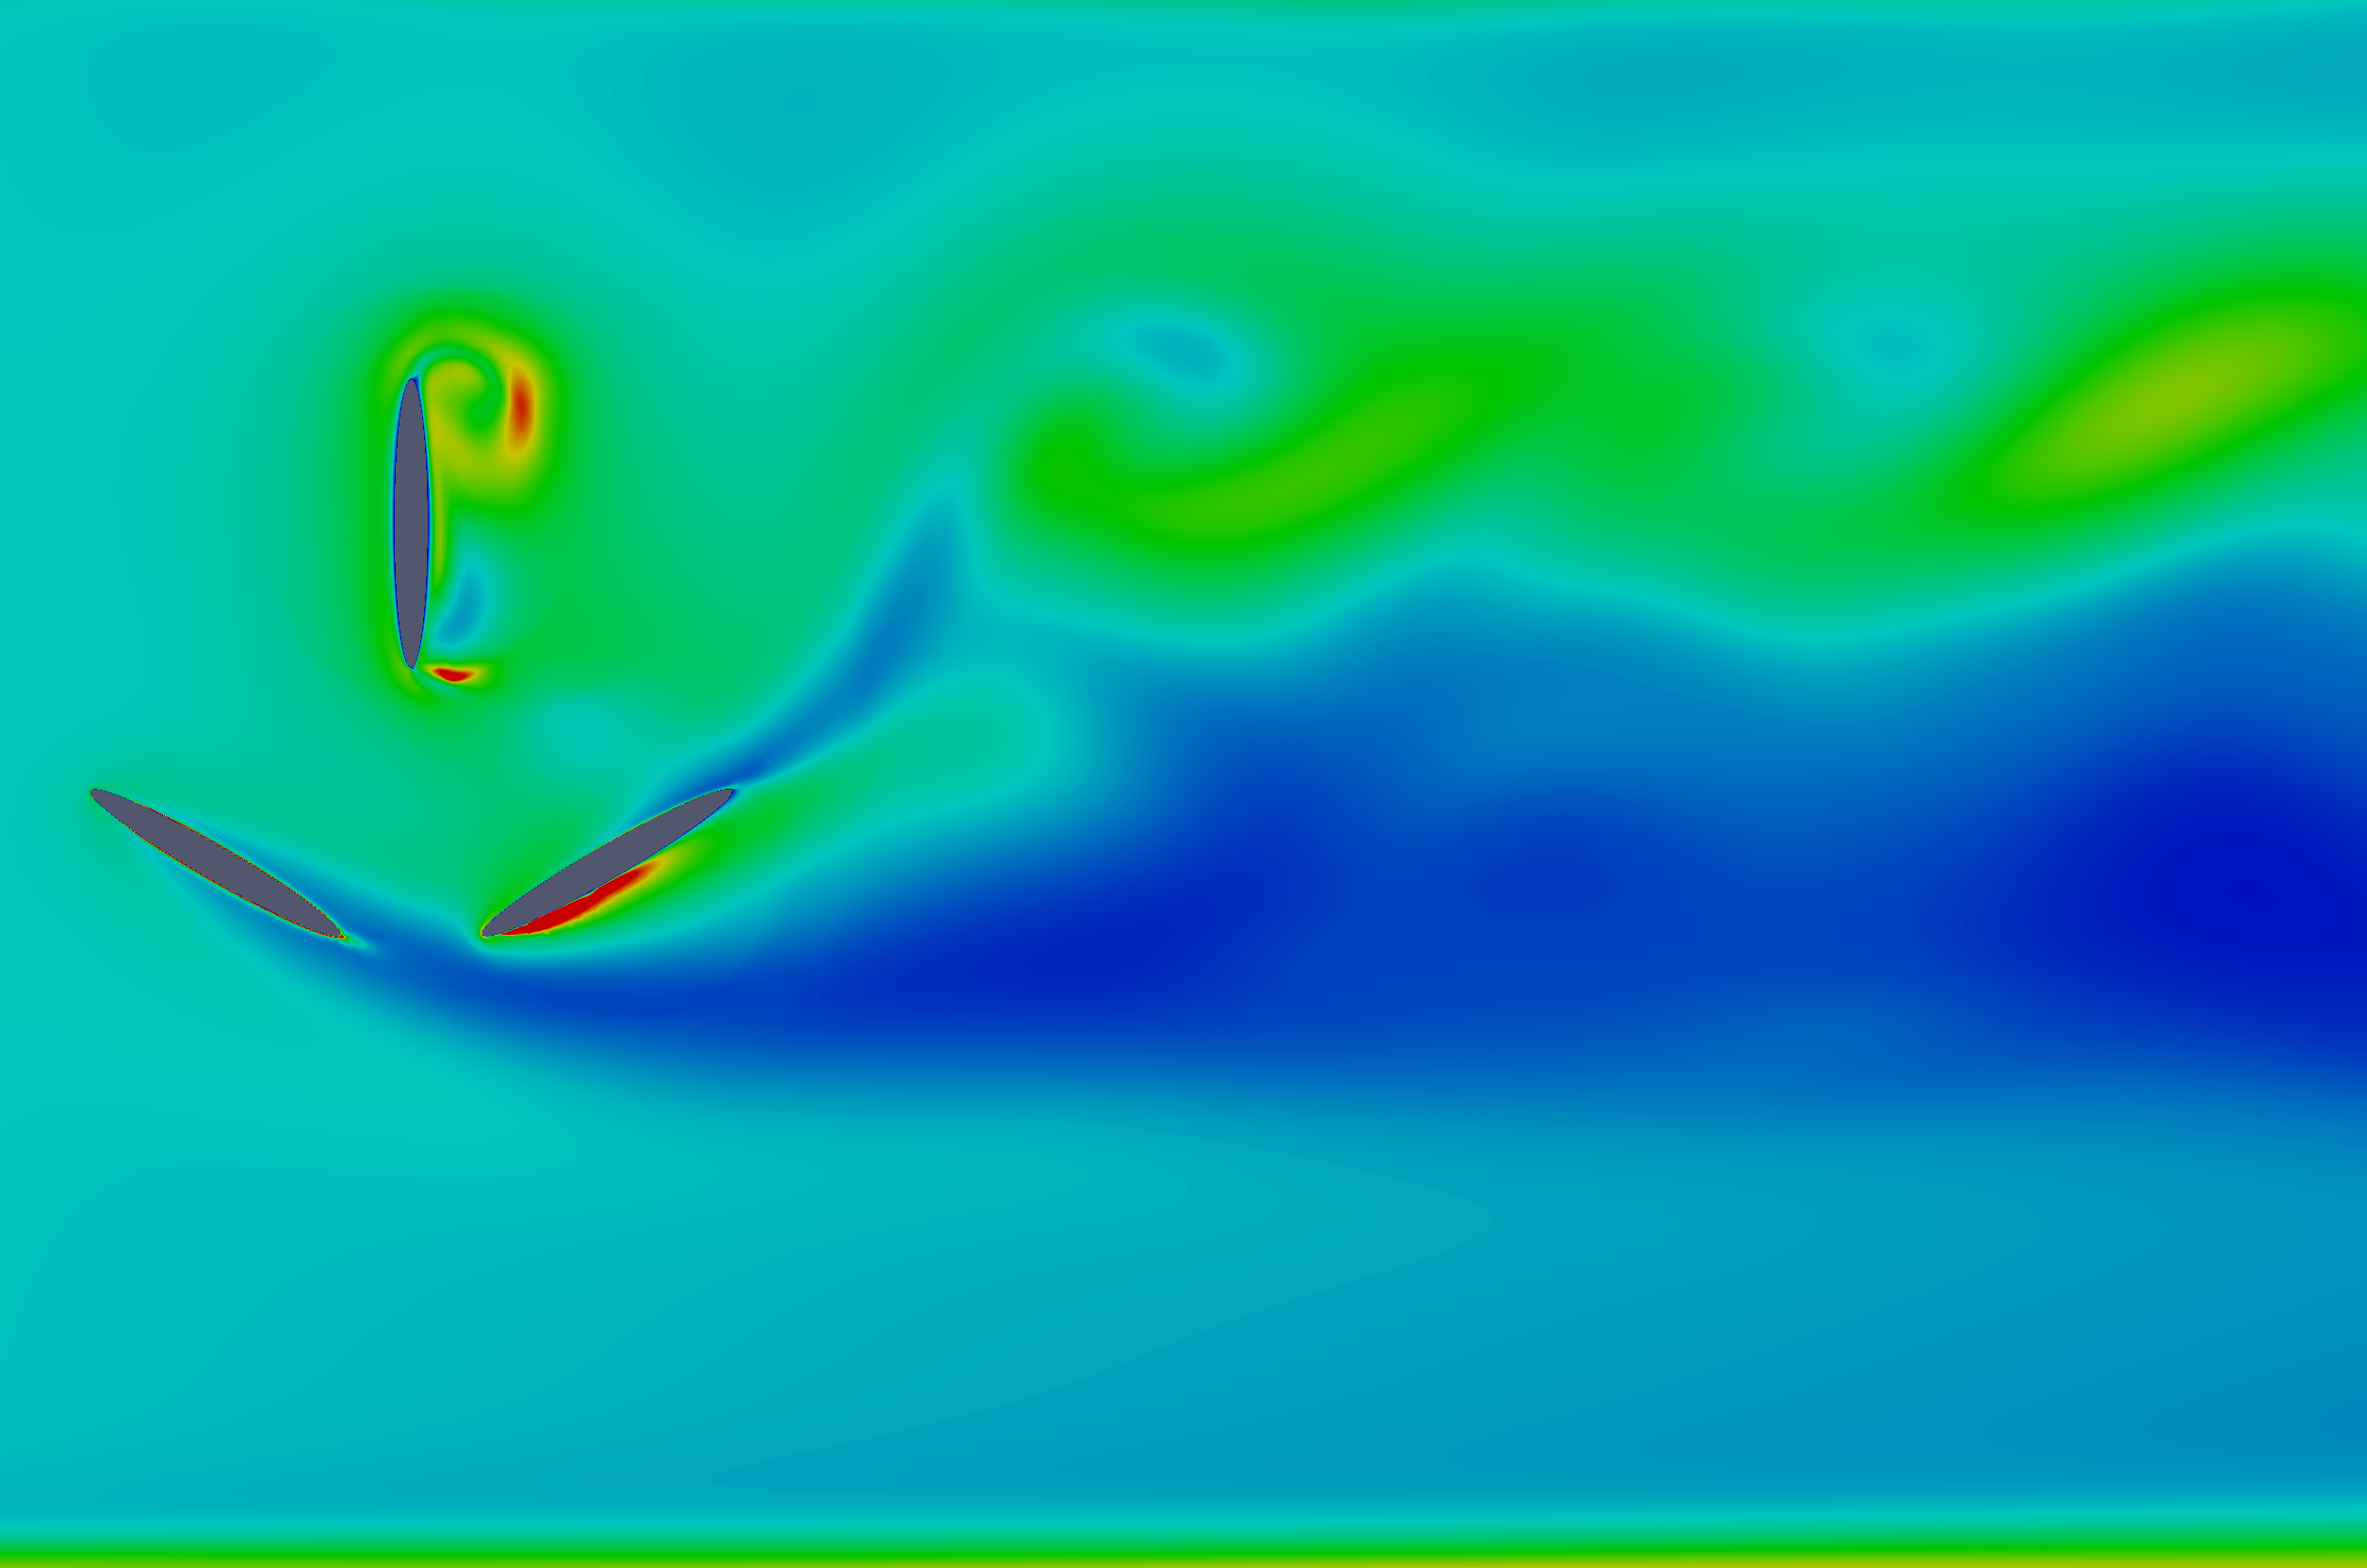
\includegraphics[width=\textwidth]{images/cover.png}
}
\date{}

% usefull for ltablex to split long tables in many pages
\keepXColumns

\DeclarePairedDelimiter\abs{\lvert}{\rvert}%

%\newcommand{\Fy}[1]{\text{F}_{y_{#1}}}

%\newcommand{\diameter}{\oslash}

%\newcommand{\todo}{\colorbox{cyan!60}{TODO}}

\renewcommand{\thesubsection}{\thesection.\arabic{subsection}}

\renewcommand{\arraystretch}{1.4}

\newcommand{\variable}[1]{\textcolor{blue}{#1}}

\newcommand{\paramtext}[1]{\textcolor{black!30!green}{#1}}

\newcommand{\terminal}[1]{\textcolor{black!30!cyan}{#1}}

\newcommand{\todo}{\colorbox{cyan!60}{TODO}}

\newcommand{\nut}{\nu_\text{T}}

\newcommand{\foam}[1]{{\ttfamily #1}}


\lstset{
	basicstyle=\fontsize{11}{13}\selectfont\ttfamily,
    frame=tb, % draw a frame at the top and bottom of the code block
    tabsize=4, % tab space width
    showstringspaces=false, % don't mark spaces in strings
    numbers=left, % display line numbers on the left
    commentstyle=\color{black!50!green}, % comment color
    keywordstyle=\color{blue!50!cyan}, % keyword color
    stringstyle=\color{black!30!red} % string color
}



\newcommand{\fakecaption}{%
  \vskip0.5\baselineskip
  \refstepcounter{table}%
  \tablename\ \thetable%
}

\makeindex

\begin{document}

\section{Turbulence}
In order to further improve the model also the turbulence model has been investigated.
Different turbulence models have been used in calculation:


\begin{enumerate}
\item Laminar model
\item $k-\varepsilon$ model
\item $k-\omega $ SST model
\end{enumerate}

\subsection{Remark on the used mesh}
The mesh which has been used is that outcoming from the mesh-sensitivity analisys.

\subsection{Comparison criterion}
It is worth noting that the assestment on the turbulence model is carried out via the evaluation of the $y^+ $ parameter which is directly related on the mesh size near the walls and on the wall shear stress.
The mesh features are mantained fixed while turbulence models have ben investigated, i.e. the mesh clustering is not a parameter in the turbulence model assestment.


\subsection{Turbulence model}

\paragraph{Laminar}
As first option the laminar model has been used in order to have a comparison tool.
It must be clarified that the physical situation that is expected is that of a turbulent motion, since the flow in evolving within a rotating blade domain; moreover the flow develops around aerodynamic profile on a wide range of angles of attach; at the end of the day what is expected is a vortical/turbulent-induced flow.\\
 

\begin{figure}[H]

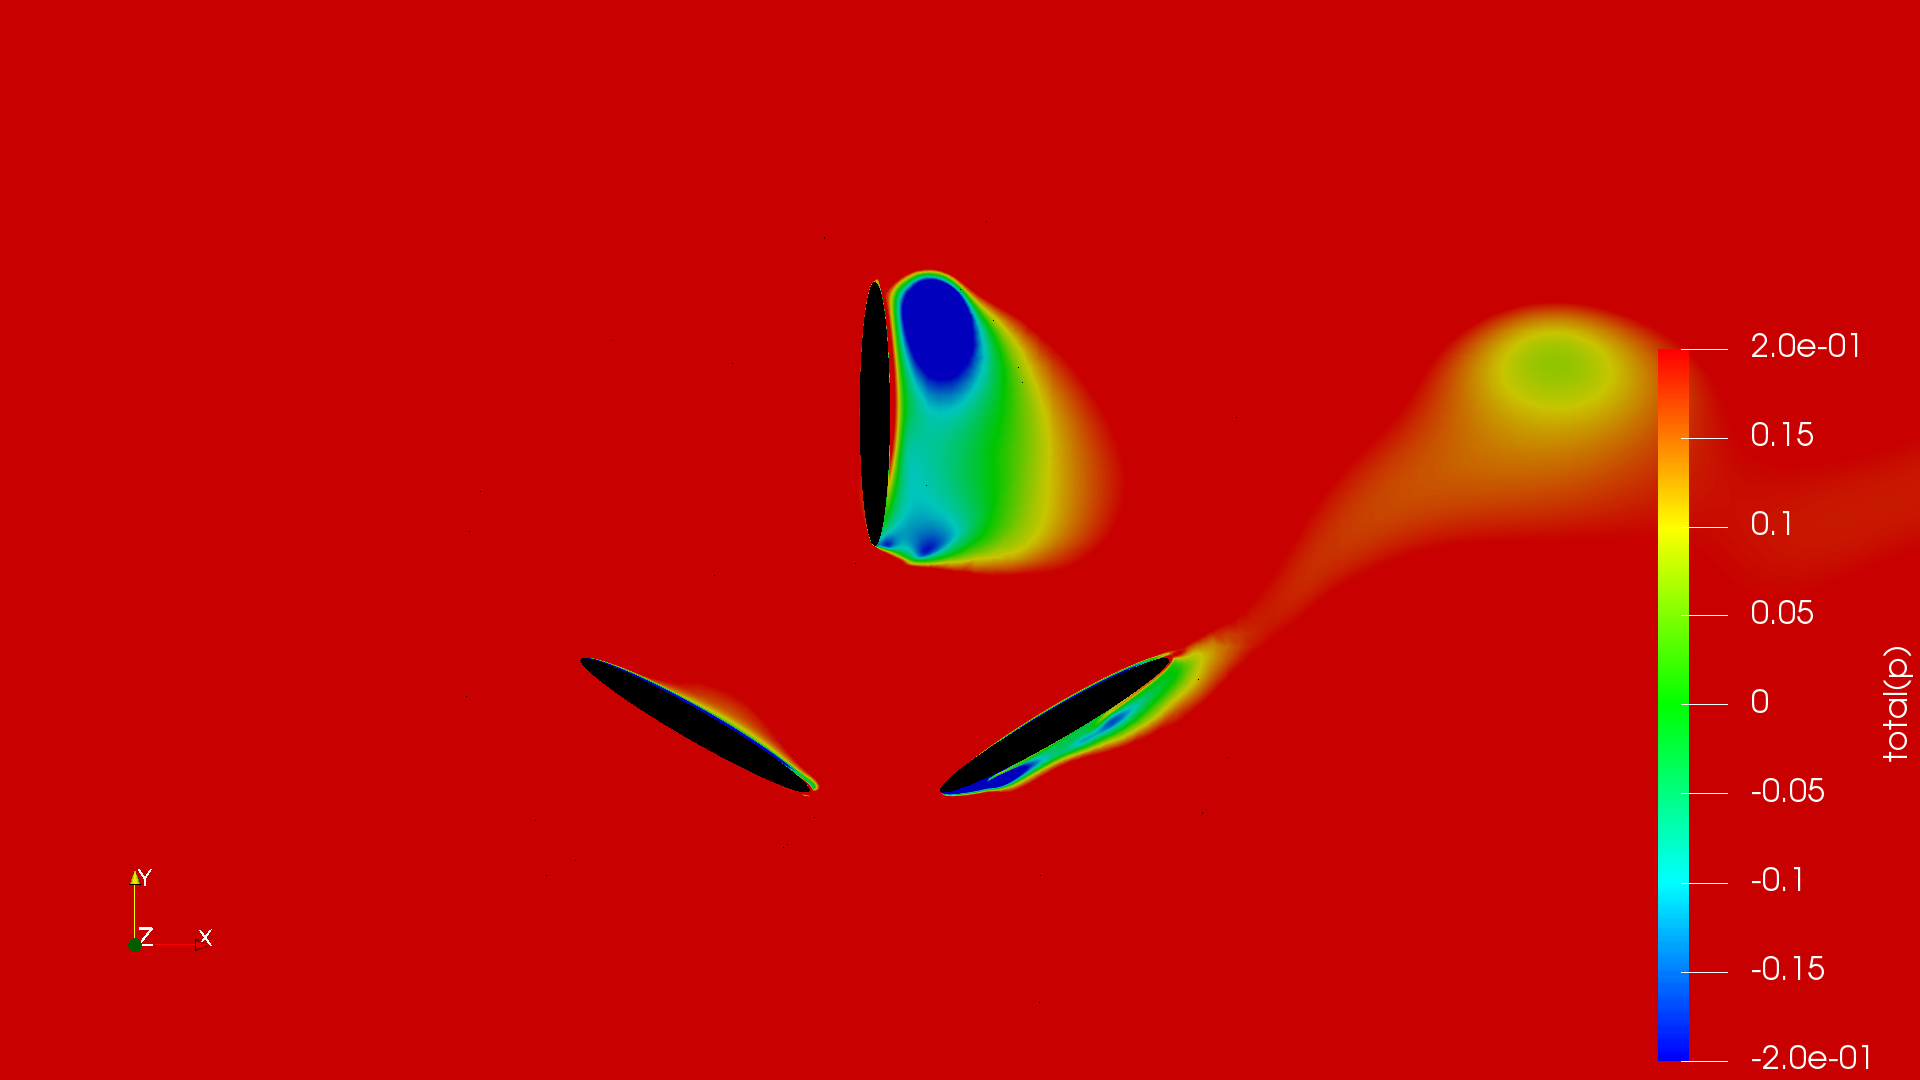
\includegraphics[width=\textwidth]{images/turbulence/laminar_pressureDrop.png} 
\caption{total pressure at t = 2.4[s] in a laminar simulation}
\centering
\end{figure}

\todo{} CERCA DETTAGLI DI DISTACCO


\paragraph{$k-\varepsilon$ model}
As first attempt for turbulence model the $k-\varepsilon$ model has been used.
The result has been assessed in term of the $y^+ $ which is computed by OpenFoam on the patch of type $wall$, namely $lower wall$, $blade0$, $blade1$ and $blade2$.\\
if the values of $y^+ $ would satisfy the condition 

\begin{equation}
\ y^+ > 30
\end{equation}

then the turbulence model would be validated; this would mean that the solver is going to solve the $k-equation $ and $\varepsilon-equation $ in the far wake region without problems of singularity and, then, take advantage ofthe wall-functions at the wall to calculate the flow field.\\
The results are presented in the following table in terms of minimum and maximum $y^+ $ for each wall at the last timestep $t = 2.4[s]$.

\begin{tabular}{r|c|c|}
&$min(y^+) $&$max(y^+) $\\ \hline
lower wall & 6.793848e-01 & 4.095234e+00\\ \hline
blade0 & \round{5.503802e-02}	 & 7.997351e-01\\ \hline
blade1 & 4.869300e-02	& 1.742530e-01\\ \hline
blade2 & 7.257931e-02	&7.748824e-01\\ \hline
\end{tabular}\\

as can be seen from the table the $y^+ $ values do not validate the choice of $k-\varepsilon$ turbulence model.\\

\paragraph{$k-\omega $ SST model}
Given the $y^+$ values, is evident that the mesh clustering near the walls of the blades is suitable for the $k-\omega-SST$ model which avoids problems of singularity of the equations and can solve directly the boundary layers of the blades.\\
Particular attention has been paid for the mesh clustering in the O-grid near the wall of the blade, it has been set properly in order to guarantee the smooth variation of flow property from the BL to the free stream.

\subsection{Turbulence models, a comparison}
A brief qualitative comparative study of the performance of the machine, given different turbulence models has been carried out.
\paragraph{Mean power}
the mean power has been compared at t=1.8[s] for all the three turbulence setups. 
\todo{} MANCA GRAFICO
\paragraph{Pressure power}
\todo{} MANCA OUTPUT
\paragraph{Shearing power}
\todo{} MANCA OUTPUT
\paragraph{Velocity profiles}
The velocity profiles outcoming from different turbulence simulations have been compared in the wake regions, i.e. where the effect of the turbulence is expected to play its major role.\\
The plotted regions are the following:\\
\todo{} INSERIRE SCREENSHOTS DELLE LOCATIONS

\todo{} INSERIRE GRAFICI
















\end{document}
